\section{Aussagenlogik}
\subsection*{Aussage}
Eine Aussage ist ein Satz, der entweder wahr oder falsch ist, also nie beides zugleich.
Wahre Aussagen haben den Wahrheitswert $w$ und falsche Aussagen den
Wahrheitswert $f$.
\begin{center}
	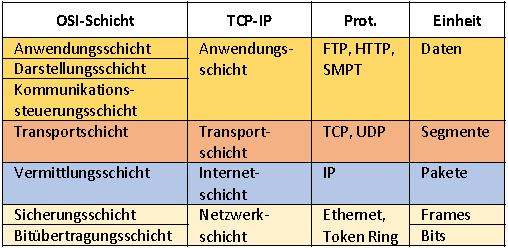
\includegraphics[width=0.8\columnwidth]{Resources/osi2.pdf}
\end{center}
\subsection*{Belegung von Variablen}
Sei $\mathcal{A}_B(F) = f$.
Dann ist stets $\mathcal{A}_B(F\Rightarrow G) = w$
\subsection*{Formelbeweis über Belegung}
Wenn $F \wedge G$ eine Tautologie ist, dann (und nur dann) ist $F$ eine Tautologie und $G$ auch.
Hinweis: In dem Lemma stecken zwei Teilaussagen, die beide zu beweisen sind:
1. Wenn $F \wedge G$ eine Tautologie ist, dann ist $F$ eine Tautologie und $G$ auch.
2. Umgekehrt: Sind $F$ und $G$ Tautologien, dann ist auch $F \wedge G$ eine.
\emph{Beweis.}
1. Annahme: $F \wedge G$ sei eine Tautologie.
Dann: Für jede Belegung $B$ wertet $F \wedge G$ zu wahr aus.
Dann: Das ist nur der Fall, wenn sowohl $F$ als auch $G$ (für jedes $B$) zu wahr auswerten.
Dann: Für jede Belegung $B$ wertet $F$ zu wahr aus. Und:
Für jede Belegung $B$ wertet $G$ zu wahr aus.
Dann: $F$ ist Tautologie und $G$ ist Tautologie.
2. Annahme: $F$ ist Tautologie und $G$ ist Tautologie.
Dann: Für jede Belegung $B_1$ wertet $F$ zu wahr aus. Und: Für jede Belegung $B_2$ wertet $G$ zu wahr aus.
Dann: Für jede Belegung $B$ wertet $F \wedge G$ zu wahr aus.
Dann: $F \wedge G$ ist eine Tautologie.
\subsection*{Äquivalenz und Folgerung}
$p\equiv q$ gilt genau dann, wenn sowohl $p\models q$ als auch $q\models p$ gelten. \emph{Beweis.}
$p\equiv q$ GDW $p\Leftrightarrow q$ ist Tautologie nach Def. von $\equiv$
GDW $(p\Rightarrow q) \wedge (q\Rightarrow p)$ ist Tautologie
GDW $(p\Rightarrow q)$ ist Tautologie und $(q\Rightarrow p)$ ist Tautologie
GDW $(p\models q)$ gilt und $q\models p$ gilt.
\subsection*{Substitution}
Ersetzt man in einer Formel eine beliebige Teilformel $F$ durch eine logisch äquivalente
Teilformel $F'$, so verändert sich der Wahrheitswerteverlauf der Gesamtformel nicht.
Man kann Formeln also vereinfachen, indem man Teilformeln durch äquivalente
(einfachere) Teilformeln ersetzt.
\subsection*{Universum}
Die freien Variablen in einer Aussagenform können durch Objekte aus einer als
Universum bezeichneten Gesamtheit wie $\mathbb{N},\mathbb{R},\mathbb{Z},\mathbb{Q}$ ersetzt werden.
\subsection*{Tautologien}
$(p\wedge q)\Rightarrow p$\text{ bzw. }$p\Rightarrow (p\vee q)$\\
$(q\Rightarrow p)\vee (\neg q\Rightarrow p)$\\
$(p\Rightarrow q)\Leftrightarrow (\neg p\vee q)$\\
$(p\Rightarrow q)\Leftrightarrow (\neg q\Rightarrow\neg p)$ \hfill\text{(Kontraposition)}\\
$(p\wedge (p\Rightarrow q))\Rightarrow q$ \hfill\text{(Modus Ponens)}\\
$((p\Rightarrow q)\wedge (q\Rightarrow r))\Rightarrow (p\Rightarrow r)$\\
$((p\Rightarrow q)\wedge (p\Rightarrow r))\Rightarrow (p\Rightarrow (q\wedge r))$\\
$((p\Rightarrow q)\wedge (q\Rightarrow p))\Leftrightarrow (p\Leftrightarrow q)$
\subsection*{Nützliche Äquivalenzen}
Kommutativität:\\
$(p \wedge q) \equiv (q \wedge p)$\\
$(p \vee q) \equiv (q \vee p)$\\
Assoziativität:\\
$(p \wedge (q \wedge r)) \equiv ((p \wedge q) \wedge r)$\\
$(p \vee (q \vee r)) \equiv ((p \vee q) \vee r)$\\
Distributivität:\\
$(p \wedge (q \vee r)) \equiv ((p \wedge q) \vee (p \wedge r))$\\
$(p \vee (q \wedge r)) \equiv ((p \vee q) \wedge (p \vee r))$\\
Idempotenz:\\
$(p \wedge p) \equiv p$\\
$(p \vee p) \equiv p$\\
Doppelnegation:\\
$\neg (\neg p) \equiv p$\\
de Morgans Regeln:\\
$\neg (p \wedge q) \equiv ((\neg p) \vee (\neg q))$\\
$\neg (p \vee q) \equiv ((\neg p) \wedge (\neg q))$\\
Definition Implikation:\\
$(p \Rightarrow q) \equiv (\neg p \vee q)$\\
Tautologieregeln:\\
$(p \wedge q) \equiv p$\hfill (falls $q$ eine Tautologie ist)\\
$(p \vee q) \equiv q$\\
Kontradiktionsregeln:\\
$(p \wedge q) \equiv q$\hfill (falls $q$ eine Kontradiktion ist)\\
$(p \vee q) \equiv p$\\
Absorptionsregeln:\\
$(p \wedge (p \vee q)) \equiv p$\\
$(p \vee (p \wedge q)) \equiv p$\\
Prinzip vom ausgeschlossenen Dritten:\\
$p \vee (\neg p) \equiv w$\\\
Prinzip vom ausgeschlossenen Widerspruch:\\
$p \wedge (\neg p) \equiv f$
\subsection*{Äquivalenzen von quant. Aussagen}
Negationsregeln:\\
$\neg\forall x:p(x)\equiv\exists x:(\neg p(x))$\\
$\neg\exists x:p(x)\equiv\forall x:(\neg p(x))$\\
Ausklammerregeln:\\
$(\forall x:p(x)\wedge\forall y:q(y))\equiv\forall z:(p(z)\wedge q(z))$\\
$(\exists x:p(x)\wedge\exists y:q(y))\equiv\exists z:(p(z)\wedge q(z))$\\
Vertauschungsregeln\\
$\forall x\forall y:p(x,y)\equiv\forall y\forall x:p(x,y)$\\
$\exists x\exists y:p(x,y)\equiv\forall y\exists x:p(x,y)$
\subsection*{Äquivalenzumformung}
Wir demonstrieren an der Formel $\neg (\neg p \wedge q) \wedge (p \vee q)$, wie man mit Hilfe der
aufgelisteten logischen Äquivalenzen tatsächlich zu Vereinfachungen kommen kann:\\
$\phantom{{}\equiv{}} \neg (\neg p \wedge q) \wedge (p \vee q)$\\
$\equiv (\neg (\neg p) \vee (\neg q)) \wedge (p \vee q)$\hfill de Morgan\\
$\equiv (p \vee (\neg q)) \wedge (p \vee q)$\hfill Doppelnegation\\
$\equiv p \vee ((\neg q) \wedge q)$\hfill Distributivtät v.r.n.l.\\
$\equiv p \vee (q \wedge (\neg q))$\hfill Kommutativtät\\
$\equiv p \vee f$\hfill Prinzip v. ausgeschl. Widerspruch\\
$\equiv p$\hfill Kontradiktionsregel
\subsection*{Quantifizierte Aussagen}
Sei $p(x)$ eine Aussageform über dem Universum $U$.
$\exists x : p(x)$ ist wahr genau dann, wenn ein $u$ in $U$ existiert, so dass $p(u)$ wahr ist.
$\forall x : p(x)$ ist wahr genau dann, wenn $p(u)$ für jedes $u$ aus $U$ wahr ist.